% \documentclass[conference]{utils/IEEEtran}
% % \documentclass{utils/sig-alternate}
% % \documentclass{utils/acm_proc_article-sp}

% \usepackage[utf8]{inputenc}
% \usepackage[T1]{fontenc}
% \usepackage{textcomp}
% \usepackage[french, english]{babel}
% \usepackage{algorithm}
% \usepackage{algpseudocode}
% \usepackage{graphicx}
% % \usepackage{hyperref}
% \usepackage{nohyperref}  % This makes hyperref commands do nothing without errors
% \usepackage{url}  % This makes \url work
% \usepackage{backnaur}

% \usepackage{tikz}
% \usepackage{pgfplots}
% \usepgfplotslibrary{external} 
% \tikzexternalize


% \usepackage[hyperref=true,%
%             url=false,%
%             isbn=false,%
%             style=numeric,%
%             maxcitenames=3,%
%             maxbibnames=100,%
%             backend=biber,%
%             block=none]{biblatex}

% \bibliography{../src/bib/OS.bib}
% \bibliography{../src/bib/Flow-Based Programming.bib}
% \bibliography{../src/bib/Functional Programming-Functional Reactive Programming.bib}
% \bibliography{../src/bib/Stream.bib}
% \bibliography{../src/bib/Dataflow.bib}
% \bibliography{../src/bib/Web & Social Networks.bib}
% \bibliography{../src/bib/Others.bib}
% \bibliography{../src/bib/Actor Model.bib}
% \bibliography{../src/bib/Misc.bib}
% \bibliography{../src/bib/Parallelisation.bib}
% \bibliography{../src/bib/Others.bib}
% \bibliography{../src/bib/Distributed Systems.bib}
% \bibliography{../src/bib/Compilation.bib}
% \bibliography{../src/bib/MyPublications.bib}
% \bibliography{../src/bib/Sync-Async.bib}
% % \bibliography{../src/bib/sigproc.bib}

% % \bibliographystyle{abbrv}
% % \bibliography{../src/bib/OS.bib,../src/bib/Flow-Based Programming.bib,../src/bib/Functional Programming-Functional Reactive Programming.bib,../src/bib/Stream.bib,../src/bib/Dataflow.bib,../src/bib/Web & Social Networks.bib,../src/bib/Others.bib,../src/bib/Actor model.bib,../src/bib/Misc.bib,../src/bib/Parallelisation.bib,../src/bib/Others.bib,../src/bib/Distributed Systems.bib}

% \input{utils/code}
% \usepackage{marginnote}
\usepackage{xcolor}
\usepackage{pifont}

\definecolor{todo}{rgb}{0.9,0.5,0.5}
\definecolor{text}{gray}{0.8}
\definecolor{red}{rgb}{1,0,0.29}
\definecolor{gray1}{rgb}{.70,.70,.70}
\definecolor{gray2}{rgb}{.75,.75,.75}
\definecolor{gray3}{rgb}{.80,.80,.80}
\definecolor{gray4}{rgb}{.85,.85,.85}
\definecolor{gray5}{rgb}{.90,.90,.90}
\definecolor{gray6}{rgb}{.95,.95,.95}

\definecolor{RED}{RGB}{255, 0, 73}
\definecolor{GREEN}{RGB}{190, 255, 0}

\newcommand{\TODO}[1]{%
  % \marginpar
  {
    \textcolor{todo}{\bf TODO}
    \textcolor{text}{#1}
  }
}

\newcommand{\ind }{%
  \hspace{4ex}%
}

\newcommand{\comment}[1]{%
  \textcolor{text}{#1}%
}

\newcommand{\nt}[1]{%
  \textcolor{red}{*}%
  \marginpar{\textcolor{red}{\fontencoding{U}\fontfamily{futs}\selectfont\char 66\relax}\vspace{3mm}\\
  \tiny{\textcolor{text}{#1}}}%
}

\newcommand{\illustration}[1]{%
  \reversemarginpar%
  \marginpar{\tiny{illustration:\\#1}}%
  \normalmarginpar%
}

\newcommand{\ftnt}[1]{%
  \footnote{\small{\url{#1}}}%
}

\newcommand{\cit}[2]{%
  \textit{``#1''}\\[-25pt]%
  \begin{flushright}%
  --- #2%
  \end{flushright}%
}


\newcommand*\rot{\rotatebox{90}}

\newcommand\lab[1]{%
  \rotatebox{90}{\parbox{3cm}{\raggedright #1}}%
}

\newlength\replength
\newcommand\repfrac{.33}
\newcommand\dashfrac[1]{\renewcommand\repfrac{#1}}
\setlength\replength{4.5pt}
\newcommand\rulewidth{1.6pt}

\newcommand\tdotfill[1][\repfrac]{\cleaders\hbox to \replength{%
  \smash{\raisebox{\arraystretch\dimexpr\ht\strutbox-.1ex\relax}{.}}}\hfill}
\newcommand\tabdotline{%
  \makebox[0pt][r]{\makebox[\tabcolsep]{\tdotfill\hfil}}\tdotfill\hfil%
  \makebox[0pt][l]{\makebox[\tabcolsep]{\tdotfill\hfil}}%
  \\[-\arraystretch\dimexpr\ht\strutbox+\dp\strutbox\relax]%
}




\newcommand{\V}{ \textcolor{green}{\ding{51}} }
\newcommand{\X}{ \textcolor{red}{\ding{53}} }
\newcommand{\U}{ \textcolor{gray}{?} }
\newcommand{\J}{ \textcolor{cyan}{\textbf{+}} }
\newcommand{\M}{ \textcolor{orange}{--} }

\newlength\callStackIndentation
\newcommand{\level}[1]{%
  \setlength\callStackIndentation{2em}%
  \hspace*{#1\callStackIndentation}%
}

\newcommand*{\circled}[1]{\tikz[baseline=(char.base)]{
            \node[shape=circle,draw,inner sep=0.8pt] (char) {#1};}}

\newcommand*{\rate}[1]{\tikz[baseline=(char.base)]{
            \colorlet{tmpcolor}{green!\the\numexpr#1*20!red}
            \node[shape=circle,inner sep=0.8pt, fill=tmpcolor] (char) {\textcolor{white}{\textbf#1}};}}

\makeatletter

\tikzstyle{chart}=[
    legend label/.style={font={\scriptsize},anchor=west,align=left},
    legend box/.style={rectangle, draw, minimum size=5pt},
    axis/.style={black,semithick,->},
    axis label/.style={anchor=east,font={\tiny}},
]

\tikzstyle{pie chart}=[
    chart,
    slice/.style={line cap=round, line join=round, very thick,draw=white},
    pie title/.style={font={\bf}},
    slice type/.style 2 args={
        ##1/.style={fill=##2},
        values of ##1/.style={}
    }
]

\tikzstyle{bar chart}=[
    chart,
    bar width/.code={
        \pgfmathparse{##1/2}
        \global\let\bar@w\pgfmathresult
    },
    bar/.style={very thick, draw=white},
    bar label/.style={font={\bf\small},anchor=north},
    bar value/.style={font={\footnotesize}},
    bar width=.75,
]

\pgfdeclarelayer{background}
\pgfdeclarelayer{foreground}
\pgfsetlayers{background,main,foreground}


\newcommand{\pie}[3][]{
    \begin{scope}[#1]
    \pgfmathsetmacro{\curA}{90}
    \pgfmathsetmacro{\r}{0.8}
    \def\c{(0,0)}
    % \node[pie title] at (90:1.3) {#2};
    \foreach \v/\s in{#3}{
        \pgfmathsetmacro{\deltaA}{\v/100*360}
        \pgfmathsetmacro{\nextA}{\curA + \deltaA}
        \pgfmathsetmacro{\midA}{(\curA+\nextA)/2}

        \path[slice,\s] \c
            -- +(\curA:\r)
            arc (\curA:\nextA:\r)
            -- cycle;
        \pgfmathsetmacro{\d}{max((\deltaA * -(.5/50) + 1) , .5)}

        \begin{pgfonlayer}{foreground}
        \path \c -- node[pos=\d,pie values,values of \s]{$\v\%$} +(\midA:\r);
        \end{pgfonlayer}

        \global\let\curA\nextA
    }
    \end{scope}
}

\newcommand{\legend}[2][]{
    \begin{scope}[#1]
    \path
        \foreach \n/\s in {#2}
            {
                  ++(0,-5pt) node[\s,legend box] {} +(3pt,0) node[legend label] {\n}
            }
    ;
    \end{scope}
}


% % Document starts
% \begin{document}

% % Title portion
% \title{
%   Transforming Javascript Event-Loop Into a Pipeline
% 	% Toward a compiler providing pipeline parallelism for the Javascript event-loop.
%   % : hide scalability constraints from the developer
% }

% \author{
% \IEEEauthorblockN{Etienne Brodu, Stéphane Frénot}\\
% \IEEEauthorblockA{\small{Univ Lyon, INSA Lyon, Inria, CITI, F-69621 Villeurbanne, France}\\
% \{etienne.brodu, stephane.frenot\}@insa-lyon.fr}\\
% \and
% \IEEEauthorblockN{Frédéric Oblé}\\
% \IEEEauthorblockA{\small{Worldline, Bât. Le Mirage,}\\
% \small{53 avenue Paul Krüger}\\
% frederic.oble@worldline.com}
% }


% % \numberofauthors{2}
% % \author{
% % \alignauthor
% % Etienne Brodu, Stéphane Frénot\\
%   % \email{\textsf{\normalsize{\{etienne.brodu, stephane.frenot\}@insa-lyon.fr}}}\\
%   % \affaddr{\textsf{\small{Univ Lyon, INSA Lyon, Inria, CITI, F-69621 Villeurbanne, France}}}
% % \and  % use '\and' if you need 'another row' of author names
% % \alignauthor
% % Frédéric Oblé\\
%   % \email{\textsf{\normalsize{frederic.oble@worldline.com}}}\\
%   % \affaddr{\textsf{\small{Worldline}}}\\
%   % \affaddr{\textsf{\small{Worldline, Bât. Le Mirage, 53 avenue Paul Krüger}}}\\
%   % \affaddr{\textsf{\small{CS 60195}}}\\
%   % \affaddr{\textsf{\small{69624 Villeurbanne Cedex}}}\\
% % }

% \maketitle

% \begin{abstract}

The development of a real-time web application often starts with a feature-driven approach allowing to quickly react to users feedbacks.
However, this approach poorly scales in performance.
Yet, the user-base can increase by an order of magnitude in a matter of hours. This first approach is unable to deal with the highest connections spikes.
It leads the development team to shift to a scalable approach often linked to new development paradigm such as dataflow programming.
This shift of technology is disruptive and continuity-threatening.
To avoid it, we propose to abstract the feature-driven development into a more scalable high-level language.
Indeed, reasoning on this high-level language allows to dynamically cope with user-base size evolutions.

We propose a compilation approach that transforms a Javascript, single-threaded real-time web application into a network of small independent parts communicating by message streams.
We named these parts \textit{fluxions}, by contraction between a flow\footnote{flux in french} and a function.
The independence of these parts allows their execution to be parallel, and to organize an application on several processors to cope with its load, in a similar way network routers do with IP traffic.
We test this approach by applying the compiler to a real web application.
We transform this application to parallelize the execution of an independent part and present the result.

\end{abstract}

\endinput

% The very short abstract 50 words

Web applications starts with a feature-oriented approach to quickly react to users feedbacks, but eventually shift to a more scalable approach.
To avoid this disruptive shift, we propose an equivalence to compile the feature-oriented approach to a scalable high-level language.
We test this approach by applying the compiler to a real web application.


% % A category with the (minimum) three required fields
% % \category{H.4}{Information Systems Applications}{Miscellaneous}
% %A category including the fourth, optional field follows...
% % \category{D.2.8}{Software Engineering}{Metrics}[complexity measures, performance measures]

% % \category{Software and its engineering}{Software notations and tools}{Compilers}[Runtime environments]

% % \terms{Compilation, dataflow, code transformation}

% % \keywords{Flow programming, Web, Javascript} % NOT required for Proceedings

% % \eject

\chapter{Fluxion} \label{chapter5}

\section{Introduction}

\section{Fluxional execution model} \label{section:model}

This section presents an execution model to provide scalability to web applications with a granularity of parallelism at the function level.
Functions are encapsulated in autonomous execution containers with their state, so as to be mobile and parallel, similarly to the actors model.
The communications are similar to the dataflow programming model, which allows to reason on the throughput of these streams, and to react to load increases \cite{Bartenstein2014}.

The fluxional execution model executes programs written in our high-level fluxionnal language, whose grammar is presented in figure \ref{fig:flx-lang}.
An application $\bnfpn{program}$ is partitioned into parts encapsulated in autonomous execution containers named \textit{fluxions} $\bnfpn{flx}$.
The following paragraphs present the \textit{fluxions} and the messaging system to carry the communications between \textit{fluxions}, and then an example application using this execution model.

\subsection{Fluxions and Messaging System}

A \textit{fluxion} $\bnfpn{flx}$ is named by a unique identifier $\bnfpn{id}$ to receive messages, and might be part of one or more groups indicated by tags $\bnfpn{tags}$.
A \textit{fluxion} is composed of a processing function $\bnfpn{fn}$, and a local memory called a \textit{context} $\bnfpn{ctx}$.

At a message reception, the \textit{fluxion} modifies its \textit{context}, and sends messages to downstream \textit{fluxions} on its output streams $\bnfpn{streams}$.
The \textit{context} stores the state on which a \textit{fluxion} relies between two message receptions.
The messaging system queues the output messages for the event loop to process them later by calling the downstream \textit{fluxions}.

In addition to message passing, the execution model allows \textit{fluxions} to communicate by sharing state between their \textit{contexts}.
The fluxions that need this synchronization are grouped with the same tag, and loose their independence.

There are two types of streams, \textit{start} and \textit{post}, which correspond to the nature of the rupture point producing the stream.
A variable created within a chain of \textit{post} streams requires more synchronization than a variable created upstream a \textit{start} stream.
The two types and implications of rupture points are further detailed in section \ref{section:compiler}.
\textit{Start} rupture points are indicated with a double arrow ($\to$ \hspace{-1.4em} $\to$ or \texttt{>>}) and \textit{post} rupture points with a simple arrow ($\to$ or \texttt{->}).

\begin{figure}[h]
\vspace{-0.6\baselineskip}
\begin{bnf*}
  \bnfprod{program}    {\bnfpn{flx} \bnfor \bnfpn{flx} \bnfsp \bnftd{eol} \bnfsp \bnfpn{program}}\\
  \bnfprod{flx}        {\bnfts{\texttt{flx}} \bnfsp \bnfpn{id} \bnfsp \bnfpn{tags} \bnfsp \bnfpn{ctx} \bnfsp \bnftd{eol} \bnfsp \bnfpn{streams} \bnfsp \bnftd{eol} \bnfsp \bnfpn{fn}}\\
  \bnfprod{tags}       {\bnfts{\texttt{\&}} \bnfsp \bnfpn{list} \bnfor \bnftd{empty string}}\\
  \bnfprod{streams}    {\bnfts{\texttt{null}} \bnfor \bnfpn{stream} \bnfor \bnfpn{stream} \bnfsp \bnftd{eol} \bnfsp \bnfpn{streams}}\\
  \bnfprod{stream}     {\bnfpn{type} \bnfsp \bnfpn{dest} \bnfsp [\bnfpn{msg}]}\\
  \bnfprod{dest}       {\bnfpn{list}}\\
  \bnfprod{ctx}        {\bnfts{\texttt{\{}} \bnfpn{list} \bnfts{\texttt{\}}}}\\
  \bnfprod{msg}        {\bnfts{\texttt{[}} \bnfpn{list} \bnfts{\texttt{]}}}\\
  \bnfprod{list}       {\bnfpn{id} \bnfor \bnfpn{id} \bnfsp \bnfts{,} \bnfsp \bnfpn{list}}\\
  \bnfprod{type}       {\bnfts{\texttt{>}\texttt{>}} \bnfor \bnfts{\texttt{-}\texttt{>}}}\\
  \bnfprod{id}         {\bnftd{Identifier}}\\
  \bnfprod{fn}         {\bnftd{Source language with~} \bnfpn{stream} \bnftd{~placeholders}}\\
\end{bnf*}
\vspace{-2.5\baselineskip}
\caption{Syntax of a high-level language to represent a program in the fluxionnal form}
\label{fig:flx-lang}
\end{figure}

\subsection{Example}

\begin{code}[js,
  caption={Example web application},
  label={lst:source}]
var app = require('express')(),
    fs = require('fs'),
    count = 0; //@\label{lst:source-counter}@

app.get('/', function handler(req, res){ //@\label{lst:source-handler}@
  fs.readFile(__filename, function reply(err, data) {
    count += 1;
    res.send(err || template(count, data)); //@\label{lst:source-send}@
  });
}); //@\label{lst:source-handler-end}@

app.listen(8080);
\end{code}

The fluxional execution model is illustrated with an example application presented in listing \ref{lst:source}.
This application reads a file, and sends it back along with a request counter.
The \texttt{handler} function, line \ref{lst:source-handler} to \ref{lst:source-handler-end}, receives the input stream of requests.
The \texttt{count} variable at line \ref{lst:source-counter} counts the requests, and needs to be saved between two messages receptions.
The \texttt{template} function formats the output stream to be sent back to the client.
The \texttt{app.get} and \texttt{res.send} functions, lines \ref{lst:source-handler} and \ref{lst:source-send}, interface the application with the clients.
Between these two interface functions is a chain of three functions to process the client requests : \texttt{app.get} $\to$ \hspace{-1.4em} $\to$ \texttt{handler} $\to$ \texttt{reply}.
This chain of functions is transformed into a pipeline, expressed in the high-level fluxionnal language in listing \ref{lst:fluxional}.
The transformation process between the source and the fluxional code is explained in section \ref{section:compiler}.

\begin{figure}[h!]
  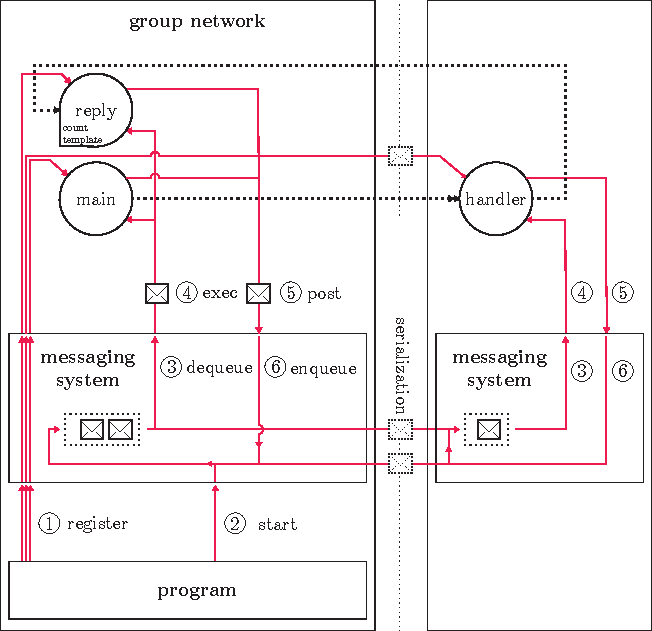
\includegraphics[width=\linewidth]{../resources/schema-message.pdf}
  \caption{The fluxionnal execution model in details}
  \label{fig:MesSys}
\end{figure}

The execution is illustrated in figure \ref{fig:MesSys}.
The dashed arrows between fluxions represent the message streams as seen in the fluxionnal application.
The plain arrows represent the operations of the messaging system during the execution.
These steps are indicated by numeroted circles.
The \textit{program} registers its fluxions in the messageing system, \circled{1}.
The fluxion \textit{reply} has a context containing the variable \texttt{count} and \texttt{tem\-plate}.
When the application receives a request, the first fluxion in the stream, \textit{main}, queues a \texttt{start} message containing the request, \circled{2}.
This first message is to be received by the next fluxion \textit{handler}, \circled{3}, and triggers its execution, \circled{4}.
The fluxion \textit{handler} sends back a message, \circled{5}, to be enqueued, \circled{6}.
The system loops through steps \circled{3} through \circled{6} until the queue is empty.
This cycle starts again for each new incoming request causing another \texttt{start} message.

\begin{code}[flx, caption={Example application expressed in the high-level fluxional language}, label={lst:fluxional}]
flx main & grp_res
>> handler [res]
  var app = require('express')(),
      fs = require('fs'),
      count = 0;

  app.get('/', >> handler); //@\label{lst:fluxional-streamtohandler}@
  app.listen(8080);

flx handler
-> reply [res]
  function handler(req, res) {
    fs.readFile(__filename, -> reply); //@\label{lst:fluxional-readfile}@
  }

flx reply & grp_res {count, template}
-> null
  function reply(error, data) {
    count += 1; //@\label{lst:fluxional-counter}@
    res.send(err || template(count, data)); //@\label{lst:fluxional-ressend}@
  }
\end{code}

The chain of functions from listing \ref{lst:source} is expressed in the fluxional language in listing \ref{lst:fluxional}.
The fluxion \texttt{handler} doesn't have any dependencies, so it can be executed in a parallel event-loop.
The fluxions \texttt{main} and \texttt{reply} belong to the group \texttt{grp\_res}, indicating their dependency over the variable \texttt{res}.
The group name is arbitrarily chosen by the compiler.
All the fluxions inside a group are executed sequentially on the same event-loop, to protect against concurrent accesses.

The variable \texttt{res} is created and consumed within a chain of \textit{post} stream.
Therefore, it is exclusive to one request and cannot be propagated to another request.
It doesn't prevent the whole group from being replicated.
However, the fluxion \texttt{reply} depends on the variable \texttt{count} created upstream the \textit{start} stream, which prevents this replication.
If it did not rely on this state, the group \texttt{grp\_res} would be stateless, and could be replicated to cope with the incoming traffic.

This execution model allows to parallelize the execution of an application as a pipeline, as with the fluxion \texttt{handler}.
And some parts are replicated, as could be the group \texttt{grp\_res}.
This parallelization improves the scalability of the application.
Indeed, as a fluxion contains its state and expresses its dependencies, it can be migrated.
It allows to adapt the number of fluxions per core to adjust the resource usage in function of the desired throughput.

Our goal, as described in the introduction, is not to propose a new high-level language but to automate the architectural shift.
We present the compiler to automate this architectural shift in the next section.
\section{Fluxionnal compiler} \label{section:compiler}

% Since 2009, \textit{Node.js} proposes an alternative to the difficult threading model adopted almost universally \cite{Adya2002}.
% % It provides a Javascript execution environment for real-time web applications.
% Its concurrency model is based on an event-loop, and exposes performances interesting enough for half the silicon valley to migrate to.
% We focus on this promising environment for its initial simplicity and efficiency.

% An event-loop executes a program on a single thread of execution.
% It avoids synchronization over the global memory, and all the problems associated.
% It features asynchronous programming to avoid wasting execution time waiting for long operations to complete, like input/output operations.
% These operations are executed in parallel, as they don't require access to the global memory.
% To resume the execution, the call to an asynchronous operation requires a callback.
% That is a function passed as a parameter of the callee to resume execution once the asynchronous operation is finished.
% Callback is a software construct present in any language with higher-order functions.

% After the operation completes, its callback is queued to be executed sequentially by the event-loop.
% A callback is loosely coupled with the caller of the asynchronous operation.
% They are not executed on the same call stack.
% This rupture marks out the separation between two independent application parts.
% The two parts are callbacks, as the caller of the asynchronous operation is itself the callback of another caller, up until the root of the program.
% The execution is organized as a tree of callbacks executed independently.
% It is a particularity of using the event-loop as a base for the concurrency model in the implementation of the execution engine.

% However, the rupture between two callbacks is not trivial.
% Languages providing higher-order functions often provide closures as the implementation of lexical scoping.
% A closure is a function that keeps the execution context of its initial definition.
% It means that the callback provided to an asynchronous function keeps access on the memory scope of the caller of this asynchronous function.
% To execute a callback in parallel, its memory needs to be independent from the global memory.
% The dependencies resulting from closures needs to be addressed, and resolved by our compiler.

The source languages we focus on should present higher-order functions and be implemented as an event-loop with a global memory.
Javascript is such a language : it doesn't require an event-loop, but it is often implemented on top of an event-loop.
\textit{Node.js} is an example of such an implementation.
We developed a compiler that transforms a \textit{Node.js} application into a fluxional application compliant with the execution model described in section \ref{section:model}.

\begin{figure}[h!]
\begin{center}
  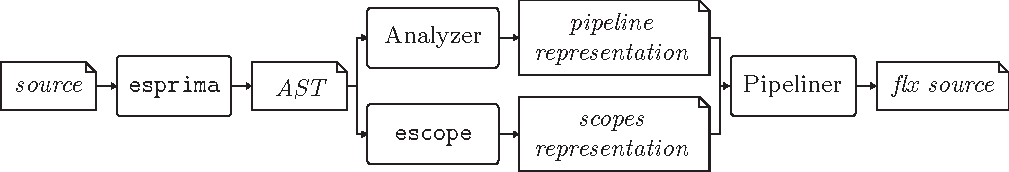
\includegraphics[width=\linewidth]{resources/compiler-stream.pdf}
  \caption{Compilation chain}
  \label{fig:compilation}
\end{center}
\end{figure}

The chain of compilation is described in figure \ref{fig:compilation}.
From the source of a \textit{Node.js} application, the compiler extracts an Abstract Syntax Tree (AST) with \texttt{esprima}.
From this AST, the analyzer step identifies the limits of the different application parts and how they relate to form a pipeline.
This first step outputs a pipeline representation of the application.
Section \ref{section:compiler:analyzer} explains this first compilation step.
In the pipeline representation, the stages are not yet independent and encapsulated into fluxions.
% From the AST, the compiler also builds a representation of the memory scopes of variables.
From the AST, \texttt{escope} produces a representation of the memory scopes.
The pipeliner step analyzes the pipeline representation and the scopes representation to distribute the shared memory into independent groups of fluxions.
Section \ref{section:compiler:pipeliner} explains this second compilation step.

% We do not target all Javascript Web-based application as this work is only a proof of concept for the compilation.
% Our goal is to compile a few real applications without modifying their code, so as to validate this approach.

\subsection{Analyzer step} \label{section:compiler:analyzer}

The limit between two application parts is defined by a rupture point.
The analyzer identifies these rupture points, and outputs a representation of the application in a pipeline form, with application parts as the stages, and rupture points as the message streams of this pipeline.

\subsubsection{Rupture points} \label{section:compiler:analyzer:rupture}

A rupture point is a call of a loosely coupled function.
It is an asynchronous call without subsequent synchronization with the caller.
In \textit{Node.js}, I/O operations are asynchronous functions and indicate such rupture point between two application parts.
Figure \ref{fig:basicrp} shows an example of a rupture point with the execution of the two application parts isolated into fluxions.
The two application parts are the caller of the asynchronous function call on one hand, and the callback provided to the asynchronous function call on the other hand.

\begin{figure}[h!]
\begin{center}
  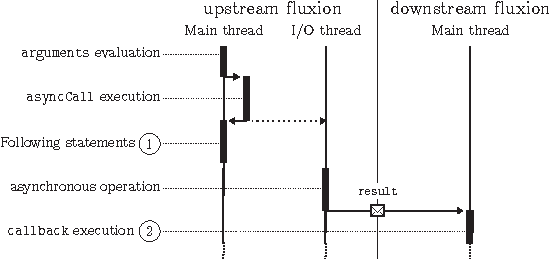
\includegraphics[width=\linewidth]{resources/basicrp.pdf}
  \begin{code}
asyncCall(arguments, function callback(result){ //@\circled{2}@ });
// Following statements //@\circled{1}@
  \end{code}
  \caption{Rupture point interface}
  \label{fig:basicrp}
\end{center}
\end{figure}

A callback is a function passed as a parameter to a function call.
It is invoked by the callee to continue the execution with data not available in the caller context.
We distinguish three kinds of callbacks, but only two are asynchronous : listeners and continuations.
% \textbf{Iterators} are functions called for each item in a set, often synchronously.
% \textbf{Listeners} are functions called asynchronously for each event in a stream.
% \textbf{Continuations} are functions called asynchronously once a result is available.
Similarly, there are two types of rupture points, respectively \textit{start} and \textit{post}.

\textbf{Start rupture points} are indicated by listeners. They are on the border between the application and the outside, continuously receiving incoming user requests.
An example of a start rupture point is in listing \ref{lst:source}, between the call to \texttt{app.get()}, and its listener \texttt{handler}.
These rupture points indicate the input of a data stream in the program, and the beginning of a chain of fluxions to process this stream.

\textbf{Post rupture points} are indicated by continuations.
They represent a continuity in the execution flow after an asynchronous operation yielding a unique result, such as reading a file, or querying a database.
An example of a post rupture points is in listing \ref{lst:source}, between the call to \texttt{fs.readFile()}, and its continuation \texttt{reply}.

% The compilation results for these rupture points is illustrated in listing \ref{lst:ex-jsres} and explained in section \ref{section:example}.

\subsubsection{Detection}

% Listeners and continuations are asynchronous because they are called asynchronously, and not because they are defined differently than any other function.
% Therefore, the identification of a rupture point holds on the callee, not on the callback.
% In listing \ref{lst:source}, the two rupture points are identified because of \texttt{app.get} and \texttt{fs.readFile}, not because of \texttt{handler} and \texttt{reply}.
% Moreover, the asynchronism is provided by the execution engine, not the language.
% It is impossible to identify an asynchronous function from a synchronous function based on their syntax.
The compiler uses a list of common asynchronous callees, like the \texttt{express} and file system methods.
This list can be augmented to match asynchronous callees individually for any application.
To identify the callee, the analyzer walks the AST to find a call expression matching this list.

% The compiler is prebuilt knowing some module names exposing asynchronous functions, like the \textit{express} and the \textit{fs} module in listing \ref{lst:rupturepoints}.
% To detect asynchronous calls, the compiler keeps a list of variables holding these modules.
% In listing \ref{lst:rupturepoints}, the compiler adds both variables \texttt{app} and \texttt{fs} in this list.
% When the compiler encounters a call expression, it compares its callee name with this list to spot asynchronous functions.

After the identification of the callee, the callback needs to be identified as well to be encapsulated in the downstream fluxion.
For each asynchronous call detected, the compiler test if one of the arguments is of type \texttt{function}.
Some callback functions are declared \textit{in situ}, and are trivially detected.
For variable identifier, and other expressions, the analyzer tries to detect their type.
To do so, the analyzer walks back the AST to track their assignations and modifications, and to determine their last value.
% It walks an intermediate representation of the source code to spot the statements modifying a variable.
% From this intermediate representation, the variable tracker builds a dependency graph which helps the analyzer to detect the type of a variable at a certain point in the execution.

% The isolation of the execution between the asynchronous call and the callback is illustrated figure \ref{fig:basicrp}.
% The interface line represent the limit between two fluxions.
% It means that the upstream fluxion sends a message to the downstream fluxion to continue the execution with the callback.


% Missing callbacks by false negatives in the detection is sub-optimal, but false positives are more critical, as they eventually introduce bugs.
% Therefore, the detection needs to be as accurate as possible to screen out false positives.
% The variable tracker is still in early development and is limited to only a few cases.
% In future works, our tracking method would be inspired from the points-to analysis \cite{Wei2014}.


\subsection{Pipeliner step} \label{section:compiler:pipeliner}

A rupture point eventually breaks the chain of scopes between the upstream and downstream fluxion.
The closure in the downstream fluxion cannot access the scope in the upstream fluxion as expected.
The pipeliner step replaces the need for this closure, allowing application parts to rely only on independent memory stores and message passing.
It determines the distribution using the scope representation, which represents the variables' dependencies between application parts.
Depending on this representation, the compiler can replace the broken closures in three different ways.
We present these three alternatives with the example figure \ref{fig:states}.

\begin{figure}[h!]
\begin{center}
  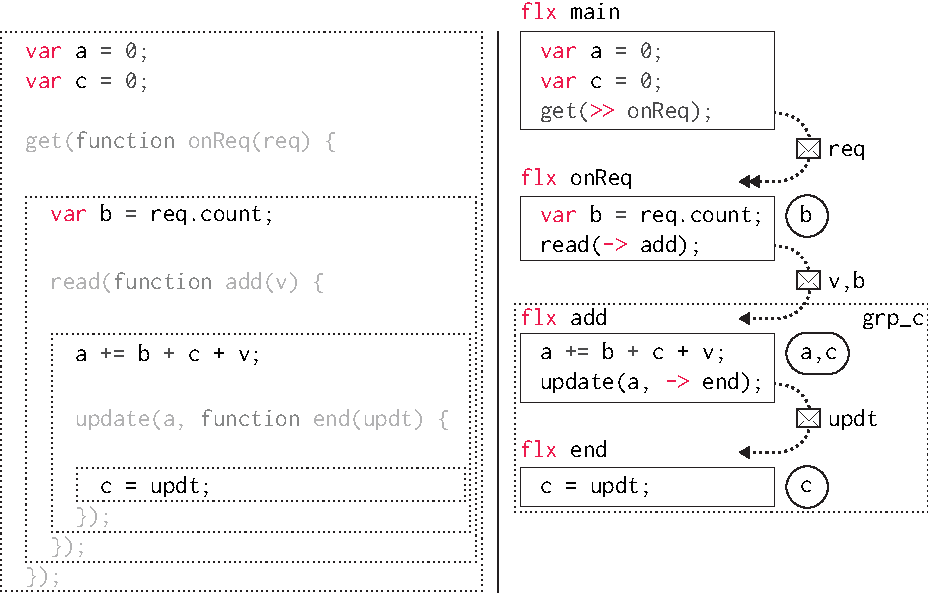
\includegraphics[width=\linewidth]{resources/states.pdf}
  \caption{Variable management from Javascript to the high-level fluxionnal language}
  \label{fig:states}
\end{center}
\end{figure}

\paragraph{Scope}
If a variable is modified inside only one application part in the current \textit{post} chain, then the pipeliner adds it to the context of its fluxion.

In figure \ref{fig:states}, the variable \texttt{a} is updated in the function \texttt{add}.
The pipeliner step stores this variable in the context of the fluxion \texttt{add}.
% The fluxion has an exclusive access to it.
% If the context of a fluxion doesn't contains references shared with other fluxions, then it can be isolated on its own worker for its execution to be parallelized.

\paragraph{Stream}
If a variable is modified inside an application part, and read inside downstream application parts, then the pipeliner makes the upstream fluxion add this variable to the message stream to be sent to the downstream fluxions.
It is impossible to send variables to upstream flux\-ions, without race conditions.
If the fluxion retro propagates the variable for an upstream fluxion to read, the upstream fluxion might use the old version while the new version is on its way.

In figure \ref{fig:states}, the variable \texttt{b} is set in the function \texttt{onReq}, and read in the function \texttt{add}.
The pipeliner step makes the fluxion \texttt{onReq} send the updated variable \texttt{b}, in addition to the variable \texttt{v}, in the message sent to the fluxion \texttt{add}.

Exceptionally, if a variable is defined inside a \textit{post} chain, like \texttt{b}, then this variable can be streamed inside this \textit{post} chain without restriction on the order of modification and read.
Indeed, the execution of the upstream fluxion for the current \textit{post} chain is assured to end before the execution of the downstream fluxion.
Therefore, no reading of the variable by the upstream fluxion happens after the modification by the downstream fluxion.
% A streamed variable is eventually in the context of an upstream fluxion, or is part of the original client request.


% Additionally, it is currently impossible to stream variables containing closures.
% Indeed, it is impossible to serialize closure from within Javascript.
% As the fluxionnal execution model is currently confined inside the Javascript execution environment, it is unable to send closures from one worker to the other.

\paragraph{Share}
If a variable is needed for modification by several application parts, or is read by an upstream application part, then it needs to be synchronized between the fluxions.
% The synchronization of a distributed memory is a well-known subject starting with the BASE semantics\cite{Fox1997}.
To respect the semantics of the source application, we cannot tolerate inconsistencies.
Therefore, the pipeliner groups all the fluxions sharing this variable within a same tag.
% Similarly, if a fluxion shares references or closures with other fluxions, either in its context, or streams, they need to be hosted on the same worker.
And it adds this variable to the contexts of each fluxions.

In figure \ref{fig:states}, the variable \texttt{c} is set in the function \texttt{end}, and read in the function \texttt{add}.
As the fluxion \texttt{add} is upstream of \texttt{end}, the pipeliner step groups the fluxion \texttt{add} and \texttt{end} with the tag \texttt{grp\_c} to allow the two fluxions to share this variable.

% \subsubsection{Higher-order language}

% Higher-order languages allow to manipulate functions like any other kind of values.
% This feature allows for the callbacks construction, but it also allows for dynamic callback evaluation
% Therefore, the pipeline representation is completed only dynamically.
% \comment{We currently limit dynamically resolved callbacks to become application parts.
% I am working to dynamically create fluxions}.


% \begin{code}
% var counter = 0;

% get(function server(request) {
%   async(handlers[request])
% })

% var handlers = {
%   'prompt' : function prompter () {
%     send(counter);
%   },
%   'buy' : function buyer () {
%     counter += 1;
%     send(counter);
%   },
%   'sell' : function seller () {
%     counter -= 1;
%     send(counter);
%   }
% }
% \end{code}

% As an example, in the code example above the compiler cannot know statically which of the \texttt{handlers} functions will be used.
% Therefore it cannot create the fluxions during compilation time.
% We modify the program to dynamically detect and create fluxion from dynamically evaluated callbacks.

% The runtime must works on graph to determine how an application can be distributed based on the dependency graph between fluxions.


\endinput





% The rupture between two callbacks is not trivial.
% Languages providing higher-order functions often provide closures as the implementation of lexical scoping.
% A closure is a function that keeps the execution context of its initial definition.
% It means that the callback provided to an asynchronous function keeps access on the memory scope of the caller of this asynchronous function.
% To execute a callback in parallel, its memory needs to be independent from the global memory.
% The dependencies resulting from closures needs to be addressed, and resolved by the second part of our compiler, the pipeliner.

% In a stream processing, there is roughly two kinds of usage of the global memory : data and state \cite{Fernandez2014a}.
% Naively, the data represent a communication channel between different application parts, and the state represents a communication channel between different instant in time.
% The data flow from stage to stage through the pipeline, and are never stored on any fluxion. In the source application, it is stored in the heap, only as a buffer between the different callbacks.
% The state, on the other hand, remains in the memory to impact the future behaviors of the application.
% State might be shared by several parts of the application.
% So, the identification of rupture points is not enough for a fluxion to be isolated, and its execution parallelized.
% The compiler also needs to analyze the memory accesses to identify which part of the state is needed by each fluxion, and allow their coordination.




% \subsubsection{Scope isolation}

% In Javascript, the memory is organized in scopes.
% They are nested one in the other up to the all-enclosing global scope.
% Each function creates a new scope containing variables local to itself.
% It is chained to the scope of the parent function, so that the child function can access variables in the scope of the parent functions, up to the global scope.
% However, the scope of the function inside a fluxion is isolated from its ancestors.

% A rupture point eventually breaks a chain of scopes.
% When it is between a child scope and its parent, it makes the child unable to access its parent as expected.
% The parent is in the upstream fluxion, and the child in the downstream fluxion.
% %For example, callback functions declared \textit{in situ}.
% Or when it is between a closure, and its definition context.
% The definition context is in the upstream fluxion and the closure in the downstream fluxion.
% If this situations aren't resolved, they introduce errors in the compilation result.
% The linker analyzes how scopes are distributed among the fluxions to identify how the variables broken onto several fluxions are used in the upstreams and downstreams fluxions.
% At the end of this analysis, the compiler knows for every variable, if it is read or modified inside each fluxion.

% However, scopes are an abstract representation of the memory, it is only the surface.
% Internally, the heap is a global memory without any fencing.
% A variable in one scope can point to the same object as another variable in another scope.
% If the first variable is modified, the modification propagates to the second variable, without this second variable being visibly modified.
% This situation produces side-effects between the two scopes.
% We call these side-effects scope leaking.
% If these two scopes are isolated on two different workers, the side-effects are unable to propagate as expected.
% We identified three basic situations leading to scope leaks.

% \paragraph{Assignment}

% If the object of a variable is assigned to another variable, there is possibly side effects between these two variables.
% It is illustrated in listing \ref{lst:assignment}.
% The variable \texttt{a} is never modified visibly, yet, it is modified through the variable \texttt{b}.

% \begin{code}[js, caption={Example of a scope leak due to assignment},label={lst:assignment}]
% var a = {item: 'unchanged'};
% var b = a;

% async_fn(function callback() {
%   b.item = 'changed';
%   console.log(a.item); // 'changed';
% })
% \end{code}

% \paragraph{Function call}

% When a variable containing an object is passed as an argument to a function call, it is assigned to a different variable as a parameter inside the function scope.
% There is possibly side effects between these two variables.
% It is illustrated in listing \ref{lst:argument}.
% The variable \texttt{a} is passed as an argument to the function \texttt{async\_fn}.
% The function \texttt{callback} is then called by \texttt{async\_fn} with the object from \texttt{a} as an argument.
% The variable \texttt{a} is never modified visibly, yet it is modified through the variable \texttt{b}.

% \begin{code}[js, caption={Example of a scope leak due to a function call},label={lst:argument}]
% var a = {item: 'unchanged'};

% async_fn(function callback(b) {
%   b.item = 'changed';
%   console.log(a.item); // 'changed';
% }, a);
% \end{code}

% \paragraph{Closure}

% When a closure is called, it can modify its creation context from outside the scope of this creation context.
% It leads to side effects from outside this scope.
% It is illustrated in listing \ref{lst:closure}.
% The variable \texttt{a} is only modified visibly inside an anonymous function.
% This anonymous function is returned to be assigned in the variable \texttt{closure}.
% The variable \texttt{a} is modified when \texttt{closure} is called.

% \begin{code}[js, caption={Example of a scope leak due to a closure},label={lst:closure}]
% function closureFactory() {
%   var a = {item: 'unchanged'};
%   return function() {
%     a.item = 'changed';
%   }
% }

% var closure = closureFactory();

% async_fn(function() {
%   closure();
%   // inside closureFactory : a.item === 'changed';
% });
% \end{code}

% Our compiler is currently in early stage of development.
% It is unable to analyze the memory deeply enough to provide a sound and complete analysis.
% Hence, the static scope analysis previously presented is unable to take these scope leaking into account.
% % Therefore it might lead to runtime errors.
% % Moreover, we present only basic situations of scope leaking.
% % Javascript exposes many other features leading to scope leaking, like prototype inheritance.
% We believe that with the right combination of static and dynamic analysis it is possible to produce a sound and complete representation of the memory.
% We leave the improvement of this analysis for future work.




















\endinput

























\subsection{Compilation example} \label{section:example}

% For copyright reason, the compiler source code is kept private along with the tests we used.
To illustrate the compiler features, we compiled the application used as an example for the execution model in section \ref{section:model}.
The source and compiled results of this application are available on github\cite{flx-example}.
The compiler source code is the property of Worldline, and is not publicly available, but we are planning of releasing it as an open source project in the future.

To test the source or the result of the compilation, one would launch respectively \texttt{source.js} or \texttt{result.js} with \texttt{node} and check the service available at \texttt{localhost:8080}.
Both executable needs their dependencies to be resolved with \texttt{npm} before execution.
\begin{verbatim}
git clone https://github.com/etnbrd/flx-example
cd flx-example
npm install
node result.js
open http://localhost:8080
\end{verbatim}

The file \texttt{source.js}, in listing \ref{lst:ex-source}, is the source of this compilation example.
This application sends back its own source along with a download counter.
The processing chain of function is : $\texttt{get} \to \texttt{handler} \to \texttt{readFile} \to \texttt{reply} \to \texttt{send}$.
It uses two asynchronous function call with \textit{in situ} callback, one to listen for user requests and one to read its own source, respectively \texttt{app.get} line 5 and \texttt{fs.read} line 6.
It uses a global variable to increment the download counter defined line 3.
This global variable is used only in the \texttt{reply} function, line 7 and 9.

\includecode{js,
  caption={Source of the compilation example},
  label={lst:ex-source}
}
{../../flx-example/source.js}

The result of the compilation into our high-level language is in the file \texttt{result.flx}, presented in listing \ref{lst:ex-flxres}.
The analyzer detects both asynchronous calls as rupture points.
The first one is a \textit{start} rupture point, associated with the \texttt{app.get} asynchronous function call which makes the callback \texttt{handler} listen for the stream of user requests. 
The second one is a \textit{post} rupture point, associated with the \texttt{fs.readFile} asynchronous function call which reads the source file and hands it to the callback \texttt{reply}.
These two rupture points result in three application parts.
The first application part is encapsulated in the root fluxion, named after the filename, \texttt{source.js}, line 1.
It initializes the system to route the user requests to the fluxion \texttt{handler-1000}, line 8.
This second fluxion reads the file, and sends the result to the next and last fluxion \texttt{reply-1001}, line 14.
We can identify the processing chain of functions in this chain of fluxion.

\begin{center}
\texttt{source.js} (\texttt{get})\\
$\downarrow$\\
\texttt{handler-1000} (\texttt{handler}, \texttt{readFile})\\
$\downarrow$\\
\texttt{reply-1001} (\texttt{reply}, \texttt{send})
\end{center}

The linker detects that the fluxion \texttt{reply-1001} needs two variable to send the result back to the user, \texttt{res} and \texttt{count}.
The variable \texttt{res} depends on the user connection and is initialized for each new request.
It needs to be part of the \textit{signature} of the message transfered to the last fluxion.
The variable \texttt{count} is global, and the \texttt{reply} function in the fluxion \texttt{reply-1001} needs to increment it at each new request.
This global variable is in the \textit{scope} of only this application part, so the compiler stores it in the \textit{context} of this fluxion.
The division by the compiler of this application is illustrated figure \ref{fig:flux-3}.
This result is very similar to the manual division illustrated figure \ref{fig:fluxions}, as expected.

\includecode{flx,
  caption={High level fluxional language result of the compilation example},
  label={lst:ex-flxres}
}
{../../flx-example/result.flx}

\begin{figure}[h!]
\begin{center}
  \includegraphics[width=\linewidth]{ressources/flux-3.pdf}
  \caption{Division of the listing \ref{lst:ex-flxres} into three application parts. This result is similar to the manual division illustrated in figure \ref{fig:fluxions}}
  \label{fig:flux-3}
\end{center}
\end{figure}

The compiler also produces an executable targeting a simple implementation of the fluxional execution model.
This result is in the file \texttt{result.js}, presented in listing \ref{lst:ex-jsres}.
The \textit{root} fluxion is not registered because it doesn't need to receive any message by another fluxion, it only initializes the application.
The two following fluxions are registered in the messaging system.
This registration encapsulates the processing function in a \texttt{capsule} function.
The \textit{special rupture points} implies the asynchronous call to be in the downstream fluxion.
The \texttt{capsule} function encapsulates the asynchronous call from a \textit{special rupture points} or the callback from \textit{basic rupture points} in a unified processing function.

The original callback is replaced with a \texttt{placeholder} function, line 3, sending the \textit{start} message to \texttt{handler-1000}.
Line 17, \texttt{handler-1000} pushes the user request \texttt{res} in the message and \texttt{post} it directly to \texttt{reply-1001}.
Because there is a special rupture point between \texttt{handler-1000} and \texttt{reply-1001}, the asynchronous call is moved to \texttt{reply-1001} and the \texttt{post} function doesn't replace the callback, like the placeholder line 3, but is directly called.
Finally, \texttt{reply-1001} receives the message containing the user request and reads the file.
The callback of this asynchronous operation, \textit{reply} function, line 27, increments the variable \texttt{counter}, line 28, and sends the reply, line 30.

\includecode{flx,
  caption={Result of the compilation example targeting the fluxional execution model},
  label={lst:ex-jsres}
}
{../../flx-example/result.js}

\subsection{Limitations}

This compiler aims at transforming a subset of Javascript web applications presenting a specific syntax and design.
In this section, we describe briefly the current limitations of our compiler and how we plan to overcome them in future works.

\begin{itemize}
  \item Variables poorly encapsulated or used too broadly tighten dependencies accross the code, and might result in a coarser division of the application.
  \item The compilation silently fails if a variable holding a callback or a module is overwritten, or not defined in the declaration.
        The variable tracker is unable to track accurately all the modification of a variable to detect these situations which may lead the compiler either to miss rupture points, or to detect non existing one.
  \item The compiler is unable to track a dynamically resolved value, even if the value is deducible statically.
        If this variable is used in a potential rupture point, the compiler screens it out.
  \item The Javascript language offers rich composition possibilities leading to many corner cases.
        The compiler is not robust enough to understand all corner cases.
        For example, the \textit{express} module is only detected if initialized like in listing \ref{lst:rupturepoints}.
\end{itemize}
There may be other limitations we aren't aware of.

The three last limitations described above are caused by the variable tracker - described in section \ref{section:analyzer} - being in an early stage of development.
We are currently in the process of improving the robustness of the compiler to extend the subset of compilable applications.

% We believe that our work will keep scalability concerns out of the way for the development team, who could then focus on the core logic of their application.
% In future developments of this project, we aim at making application dynamically reactive to the load of user requests.
% By monitoring only the input stream, the \texttt{start} rupture points, we believe it is possible to infer the load propagation through the application.
% Using analogy with fluid dynamics, each fluxion is like a pipe, traversed by a fluid of user requests.
% The input and output throughput of this pipe could be calibrated before production use, generating an approximative model of the application reaction to input load.
% Using this model, we want to make the application's reorganize itself in a cluster to handle pikes in the user request throughput.

\section{Real case test} \label{section:evaluation}

The goal of this test is to prove the possibility for an application to be compiled into a network of independent parts.
We want to show the current limitations of this isolation and the modifications needed on the application to circumvent these limitations.
% TODO -> and finally, we present the possibilities of future works.
% We want to show the limitations of this isolation for future works, and the modifications needed to circumvent these limitations.

We present a test of our compiler on a real application, gifsockets-server\ftnt{https://github.com/twolfson/gifsockets-server}.
% This application is part of the selection from our previous paper \cite{Brodu2015}.
% We chosed it because it is a working application, simple enough to illustrate this evaluation.
This application was selected from the \texttt{npm} registry because it depends on \texttt{express}, it is tested, working, and simple enough to illustrate this evaluation.
It is part of the selection from a previous work. %\cite{Brodu2015}.

This application is a real-time chat using gif-based communication channels.
% The client sends a request containing a text typed by the user.
The server transforms the received text into a gif frame, and pushes it back to a never-ending gif to be displayed on the client.
Listing \ref{lst:gifsocket} is a simplified version of this application.

\begin{code}[js, caption={Simplified version of gifsockets-server},label={lst:gifsocket}]
var express = require('express'),
    app = express(),
    routes = require('gifsockets-middleware'), //@\label{lst:gifsocket:gif-mw}@
    getRawBody = require('raw-body');

function bodyParser(limit) { //@\label{lst:gifsocket:bodyParser}@
  return function saveBody(req, res, next) { //@\label{lst:gifsocket:saveBody}@
    getRawBody(req, { //@\label{lst:gifsocket:getRawBody}@
      expected: req.headers['content-length'],
      limit: limit
    }, function (err, buffer) { //@\label{lst:gifsocket:callback}@
      req.body = buffer;
      next(); //@\label{lst:gifsocket:next}@
    });
  };
}

app.post('/image/text', bodyParser(1 * 1024 * 1024), routes.writeTextToImages); //@\label{lst:gifsocket:app.post}@
app.listen(8000);
\end{code}

% The web application framework used in this application, \textit{express}, allows to register chains of functions to process user requests.
On line \ref{lst:gifsocket:app.post}, the application registers two functions to process the requests received on the url \texttt{/image/text}.
The closure \texttt{saveBody}, line \ref{lst:gifsocket:saveBody}, returned by \texttt{bodyParser}, line \ref{lst:gifsocket:bodyParser}, and the method \texttt{routes.write\-Text\-To\-Images} from the external module \texttt{gifsockets-middleware}, line \ref{lst:gifsocket:gif-mw}.
The closure \texttt{saveBody} calls the asynchronous function \texttt{getRawBody} to get the request body.
Its callback handles the errors, and calls \texttt{next} to continue processing the request with the next function, \texttt{routes.write\-Text\-To\-Images}.

% The closure \texttt{saveBody} gather the whole request, and let \textit{express} call the next function in the chain, \texttt{routes.write\-Text\-To\-Images}, by calling \texttt{next}, line \ref{lst:gifsocket:next}.


\subsection{Compilation}

We compile this application with the compiler detailed in section \ref{section:compiler}.
% The function \texttt{getRawBody}, line \ref{lst:gifsocket:getRawBody}, is asynchronous.
The function call \texttt{app.post}, line \ref{lst:gifsocket:app.post}, is a rupture point.
However, its callbacks, \texttt{bodyParser} and \texttt{routes.write\-Text\-To\-Images} are evaluated as functions only at runtime.
For this reason, the compiler ignores this rupture point, to avoid interfering with the evaluation.
% For future works, we intend to improve the compiler with a runtime part, to detect callbacks dynamically evaluated.
% \comment{TODO move this sentence into a future works paragraph, or explain more here ?}

The compilation result is in listing \ref{lst:flx-gifsocket}.
The compiler detects a rupture point : the function \texttt{getRawBody} and its anonymous callback, line \ref{lst:gifsocket:callback}.
It encapsulates this callback in a fluxion named \texttt{anonymous\-\_1000}.
The callback is replaced with a stream placeholder to send the message stream to this downstream fluxion.
The variables \texttt{req}, and \texttt{next} are appended to this message stream, to propagate their value from the \texttt{main} fluxion to the \texttt{anonymous\-\_1000} fluxion.
% These variables are declared in the \texttt{main} fluxion, therefore, it adds them in the stream to the downstream fluxion \texttt{anonymous\-\_1000}.

% The compilation result needs to be modified manually to fix some mistakes.
% These mistakes comes from the compiler being unstable, and in early stages of development, but most of these mistakes could be avoided in the future.
% The modified and simplified compilation result is in listing \ref{lst:flx-gifsocket}.

When \texttt{anonymous\-\_1000} is not isolated from the \texttt{main} fluxion, the compilation result works as expected.
The variables used in the fluxion, \texttt{req} and \texttt{next}, are still shared between the two fluxions.
Our goal is to isolate the two fluxions, to be able to safely parallelize their executions.

\begin{code}[flx, caption={Compilation result of gifsockets-server},label={lst:flx-gifsocket}]
flx main
>> anonymous_1000 [req, next]
  var express = require('express'),
      app = express(),
      routes = require('gifsockets-middleware'), //@\label{lst:flx-gifsocket:gif-mw}@
      getRawBody = require('raw-body');

  function bodyParser(limit) { //@\label{lst:flx-gifsocket:bodyParser}@
    return function saveBody(req, res, next) { //@\label{lst:flx-gifsocket:saveBody}@
      getRawBody(req, { //@\label{lst:flx-gifsocket:getRawBody}@
        expected: req.headers['content-length'], //@\label{lst:flx-gifsocket:req.headers}@
        limit: limit
      }, >> anonymous_1000);
    };
  }

  app.post('/image/text', bodyParser(1 * 1024 * 1024), routes.writeTextToImages); //@\label{lst:flx-gifsocket:app.post}@
  app.listen(8000);

flx anonymous_1000
-> null
  function (err, buffer) { //@\label{lst:flx-gifsocket:callback}@
    req.body = buffer; //@\label{lst:flx-gifsocket:buffer}@
    next(); //@\label{lst:flx-gifsocket:next}@
  }
\end{code}

\subsection{Isolation}

In listing \ref{lst:flx-gifsocket}, the fluxion \texttt{anonymous\_1000} modifies the object \texttt{req}, line \ref{lst:flx-gifsocket:buffer}, to store the text of the received request, and it calls \texttt{next} to continue the execution, line \ref{lst:flx-gifsocket:next}.
These operations produce side-effects that should propagate in the whole application, but the isolation prevents this propagation.
Isolating the fluxion \texttt{anonymous\_1000} produces runtime exceptions.
We detail in the next paragraph, how we handle this situation to allow the application to be parallelized.
This test highlights the current limitations of the compiler, and presents future works to circumvent them.

\subsubsection{Variable \texttt{req}}

The variable \texttt{req} is read in fluxion \texttt{main}, lines \ref{lst:flx-gifsocket:getRawBody} and \ref{lst:flx-gifsocket:req.headers}.
Then it is associated in fluxion \texttt{anonymous\_1000} to \texttt{buffer}, line \ref{lst:flx-gifsocket:buffer}.
The compiler is unable to identify further usages of this variable.
However, the side effect resulting from this association impacts a variable in the scope of the next callback, \texttt{routes.writeTextToImages}.
We modified the application to explicitly propagate this side-effect to the next callback through the function \texttt{next}.
We explain further modification of this function in the next paragraph.

% For future works, instead of relying only on the source code, we intend to analyze the memory deeper to detect such side-effects.
% \comment{TODO move this sentence into a future works paragraph, or explain more here ?}

\subsubsection{Closure \texttt{next}}

The function \texttt{next} is a closure provided by the \texttt{express} \texttt{Router} to continue the execution with the next function to handle the client request.
Because it indirectly relies on network sockets, it is impossible to isolate its execution with the \texttt{anonymous\-\_1000} fluxion.
Instead, we modify \texttt{express}, so as to be compatible with the fluxional execution model.
We explain the modification below.% , and illustrate them in listing \ref{lst:mflx-gifsocket}.
% The \texttt{req} and \texttt{next} objects needs to stay on the master worker to preserve their closures.

\begin{code}[flx, caption={Simplified modification on the compiled result},label={lst:mflx-gifsocket}]
flx main & express
>> anonymous_1000 [req, next]
  var express = require('express'),
      app = express(),
      routes = require('gifsockets-middleware'), //@\label{lst:mflx-gifsocket:gif-mw}@
      getRawBody = require('raw-body');

  function bodyParser(limit) { //@\label{lst:mflx-gifsocket:bodyParser}@
    return function saveBody(req, res, next) { //@\label{lst:mflx-gifsocket:saveBody}@
      getRawBody(req, { //@\label{lst:mflx-gifsocket:getRawBody}@
        expected: req.headers['content-length'], //@\label{lst:mflx-gifsocket:req.headers}@
        limit: limit
      }, >> anonymous_1000);
    };
  }

  app.post('/image/text', bodyParser(1 * 1024 * 1024), routes.writeTextToImages); //@\label{lst:mflx-gifsocket:app.post}@
  app.listen(8000);

flx anonymous_1000
-> express_dispatcher
  function (err, buffer) { //@\label{lst:mflx-gifsocket:callback}@
    req.body = buffer; //@\label{lst:mflx-gifsocket:buffer}@
    next_placeholder(req, -> express_dispatcher); //@\label{lst:mflx-gifsocket:next-placeholder}@
  }

flx express_dispatcher & express //@\label{lst:mflx-gifsocket:express-dispatcher}@
-> null
  merge(req, msg.req);
  next(); //@\label{lst:mflx-gifsocket:next}@
\end{code}

Originally, the function \texttt{next} is the continuation to allow the anonymous callback on line \ref{lst:gifsocket:callback}, to continue the execution with the next function to handle the request.
To isolate the anonymous callback, this function is replaced on both ends.
The result of this replacement is illustrated in listing \ref{lst:mflx-gifsocket}.
The \texttt{express} \texttt{Router} registers a fluxion named \texttt{express\-\_dispatcher}, line \ref{lst:mflx-gifsocket:express-dispatcher}, to continue the execution after the fluxion \texttt{anonymous\-\_1000}.
This fluxion is in the same group \texttt{express} as the \texttt{main} fluxion, hence it has access to network sockets, to the original variable \texttt{req}, and to the original function \texttt{next}.
The call to the original \texttt{next} function in the anonymous callback is replaced by a placeholder to push the stream to the fluxion \texttt{express\-\_dispatcher}, line \ref{lst:mflx-gifsocket:next-placeholder}.
The fluxion \texttt{express\-\_dispatcher} receives the stream from the upstream fluxion \texttt{anonymous\-\_1000}, merges back the modification in the variable \texttt{req} to propagate the side effects, before calling the original function \texttt{next} to continue the execution, line \ref{lst:mflx-gifsocket:next}.

%  to holds these objects on the master worker, and receives the result of the isolated fluxion \texttt{anonymous\_1000}.


% The application sends the original object to the fluxion \texttt{express\_dispatcher} and serialized copies to the isolated fluxion \texttt{anonymous\_1000}.
% In this latter fluxion, the anonymous callback do its computation ; it assigns the received \texttt{body} as an attribute of \texttt{req}.

% In the original application, the anonymous callback finishes by calling the function \texttt{next} to let the \texttt{Router} call the next function to process the request.
% In the compiled application, this function \texttt{next} is not available on the isolated worker.
% Instead, the anonymous callback inside \texttt{anonymous\-\_1000} calls a function \texttt{next} specially provided by the fluxional execution model to send a message to the fluxion \texttt{express\-\_dispatcher} with the modified copies of \texttt{req} and \texttt{res}.
% and call the original function \texttt{next} on the master worker.

% In the original application, \textit{express} relies on side-effects on the objects \texttt{req} and \texttt{res} to get their modifications.
% The call to \texttt{next} doesn't need them as argument.
% In the isolated fluxion, as the serialized object and their originals are isolated from each other, side-effects don't propagate.
% The special \texttt{next} function needs explicit references to the modified objects to send them back to \texttt{express\_dispatcher}.
% The fluxion \texttt{express\_dispatcher} then merges back the modified copies and their originals, before calling the original function \texttt{next}.

After the modifications detailed above, the server works as expected for the subset of functionalities we modified.
The isolated fluxion correctly receives, and returns its serialized messages.
The client successfully receives a gif frame containing the text.

\subsection{Future works}

We intend to implement the compilation process presented into the runtime.
A just-in-time compiler would allow to identify callbacks dynamically evaluated, and to analyze the memory to identify side-effects propagations instead of relying only on the source code.
Moreover, this memory analysis would allow the closure serialization required to compile application using higher-order functions.

% \subsubsection{Fluxional web framework}

% In case of error, the anonymous callback calls \texttt{res.writeHead} and \texttt{res.end}.
% These two closures are similar to the closure \texttt{next}.
% It is possible to extend the modifications presented above to build a complete web application framework, with some limitations detailed below.
% Indeed, the evaluation proves that it is possible to modify the \textit{express} framework to be compatible with the fluxional execution model.

% The closure \texttt{next} is assured to be called only once at the end of the callback.
% It can be called asynchronously, and can be assimilated to a rupture point.
% Therefore, it is safe to replace it by a communication between the two workers.
% On the other hand, the functions \texttt{res.writeHead} and \texttt{res.end} are synchronous.
% It is unsafe to replace every call by a communication between the two workers.
% It would lead to race conditions.
% These calls needs to modify the serialized, local copies of \texttt{req} and \texttt{res}, and sends the result to the master only once.

